\chapter{Architecture fonctionnelle cible du Smart WMS}

\label{chap:4}

Les chapitres précédents ont permis de passer du benchmark des solutions WMS leaders à une cartographie structurée des besoins et des cas d’usage. Ce chapitre consolide ces résultats sous la forme d’une architecture fonctionnelle cible. L’objectif n’est pas encore de choisir une technologie de déploiement, un framework ou une base de données particulière, mais de définir les responsabilités qui doivent exister dans le système, les relations entre les grands domaines métier et les conditions dans lesquelles les capacités avancées peuvent être activées.


La version présentée ici reprend l’architecture fonctionnelle élaborée pendant le stage dans son intégralité. Elle distingue les systèmes externes, le cœur opérationnel du WMS, la gestion des tâches et des travaux, les données de référence et le stockage opérationnel ou analytique, les ressources et infrastructures, l’intelligence et l’aide à la décision, puis les terminaux et appareils de terrain. Cette décomposition permet de conserver une lecture métier claire tout en préparant la future architecture applicative.


% Original : page 25, section 4.1

\section{Principes de conception}

\label{sec:4.1}

La conception repose d’abord sur la généricité. L’architecture doit rester applicable à un entrepôt disposant principalement de terminaux RF et de scanners, mais aussi à un site plus automatisé utilisant convoyeurs, AS/RS, AMR/AGV, RFID ou systèmes WCS/WES. Elle ne doit donc pas supposer qu’une technologie donnée est présente partout. Le socle fonctionnel est stable ; les mécanismes d’optimisation et les équipements avancés sont ajoutés lorsque le contexte les justifie.


Le deuxième principe est la continuité entre décision et exécution. Une prévision de charge, une proposition de slotting ou une détection de dérive énergétique n’apporte de valeur que si elle peut conduire à une action : création ou réordonnancement d’une tâche, changement de priorité, alerte, instruction vers un système externe ou intervention humaine. Cette orientation prolonge directement les enseignements du benchmark : Manhattan met en avant la connexion entre décision et exécution, SAP la richesse du contexte métier, et Oracle la centralité de l’orchestration des tâches \cite{ref4,ref5,ref6,ref7,ref8,ref9,ref10}.


Enfin, l’architecture conserve une distinction explicite entre trois niveaux. Les fonctions Core sont indispensables au WMS. Les capacités Smart améliorent une décision grâce aux données, à l’optimisation ou à la prédiction. Les capacités Optional dépendent d’une infrastructure particulière, par exemple une caméra 3D, un lecteur RFID, un robot mobile ou un BMS/EMS. Cette distinction évite de confondre transformation intelligente et automatisation systématique.


% Original : page 25, section 4.2

\section{Vue d’ensemble de l’architecture proposée}

\label{sec:4.2}

La figure 4.1 présente la vue d’ensemble. La lecture se fait du haut vers le bas. Les systèmes externes apportent des commandes, ordres, informations de transport et référentiels. Le cœur WMS exécute les processus d’entrepôt. Le moteur de tâches transforme les décisions en travail exécutable. Les ressources et infrastructures représentent les personnes, équipements, actifs et systèmes de contrôle nécessaires à cette exécution. La couche d’intelligence intervient de manière transversale pour prévoir, optimiser ou détecter. Les terminaux et dispositifs terrain assurent enfin le lien entre le système numérique et le flux physique.



% Original : page 26, section 4.3

\section{Systèmes externes et périmètre d’intégration}

\label{sec:4.3}

La première couche regroupe les systèmes qui échangent avec le WMS sans appartenir à son cœur opérationnel. L’ERP/SAP fournit notamment les commandes, informations clients et fournisseurs et certains référentiels. Le MES intervient lorsque l’entrepôt est lié à la production. Le TMS/YMS transmet les informations de transport, de rendez-vous, de camions, de quais et de statuts. Les fournisseurs apportent les ASN et informations de livraison, tandis que les clients alimentent la demande à travers les commandes et confirmations. D’autres systèmes, par exemple Finance, RH, BI ou CRM, peuvent compléter ce contexte.


Lorsque l’entreprise dispose d’un BMS/EMS, celui-ci est considéré comme une intégration externe spécialisée. Le WMS peut détecter une contrainte métier ou recommander une action liée à la température, à l’éclairage ou à l’énergie, mais l’exécution physique de la consigne reste sous la responsabilité du système bâtiment ou énergétique. Cette séparation clarifie le périmètre du Smart WMS et évite de lui attribuer des responsabilités de contrôle industriel qu’il ne doit pas nécessairement porter.


% Original : page 26, section 4.4

\section{Cœur opérationnel du WMS}

\label{sec:4.4}

Le cœur opérationnel constitue la partie indispensable de l’architecture. Il couvre six domaines. La Réception marchandises traite les rendez-vous, la réception, les contrôles qualitatifs et quantitatifs, le cross-docking et les retours fournisseurs. Le Stockage \& Inventaire gère emplacements, stocks, réapprovisionnements, stock de réserve, inventaire tournant, lots, dates et ajustements. La Gestion des commandes transforme la demande en ordonnancement, planification, waves, allocations et priorités. L’Exécution entrepôt couvre le picking, le packing, le staging, la consolidation, le chargement, l’expédition et les retours clients. Yard \& Quais organise la cour, les portes, quais et transporteurs. Enfin, les Données de référence structurent les produits, clients, fournisseurs, emplacements, unités logistiques, règles et rôles.


À ce niveau, l’objectif n’est pas d’introduire une intelligence artificielle dans chaque processus. Il est d’obtenir un socle cohérent et traçable. Une optimisation de parcours n’a de sens que si les emplacements et les tâches sont correctement modélisés ; une prévision de rupture n’est fiable que si les mouvements de stock sont correctement capturés. Le Smart WMS reste donc d’abord un WMS fonctionnellement solide.


\clearpage
\thispagestyle{plain}
\begin{figure}[p]
\centering
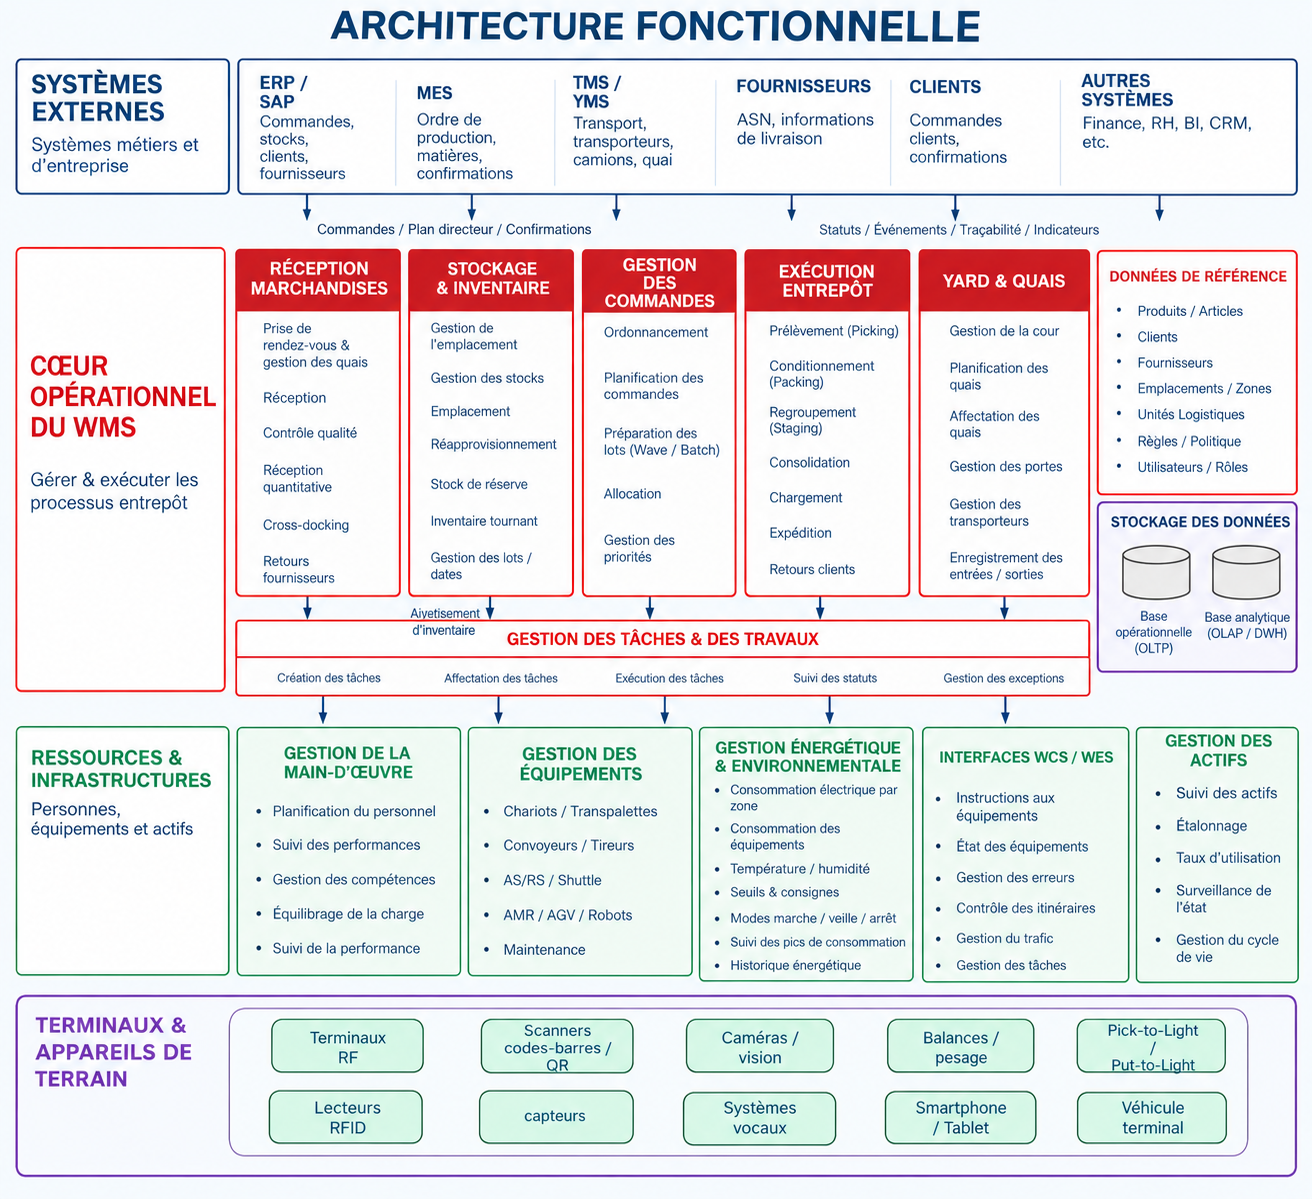
\includegraphics[width=\linewidth,height=.86\textheight,keepaspectratio]{../Architecture_f.png}
\caption{Architecture fonctionnelle cible du Smart WMS.}
\label{fig:architecture}
\end{figure}
\clearpage

\clearpage
\thispagestyle{plain}
\begin{figure}[p]
\centering
\resizebox{\linewidth}{!}{\begin{tikzpicture}[x=1cm,y=-1cm]
\pband{0}{SYSTÈMES EXTERNES}{Navy}
\pblock{0}{.35}{5.1}{1.85}{Navy}{ERP / SAP}{Commandes et stocks\par Clients et fournisseurs}
\pblock{5.45}{.35}{5.1}{1.85}{Navy}{MES}{Ordres de production\par Matières et confirmations}
\pblock{10.9}{.35}{5.1}{1.85}{Navy}{TMS / YMS}{Transport et transporteurs\par Camions et quais}
\pblock{0}{2.45}{5.1}{1.85}{Navy}{Fournisseurs}{Avis d’expédition (ASN)\par Informations de livraison}
\pblock{5.45}{2.45}{5.1}{1.85}{Navy}{Clients}{Commandes clients\par Confirmations}
\pblock{10.9}{2.45}{5.1}{1.85}{Navy}{Autres systèmes}{Finance, RH, BI, CRM\par BMS / EMS si disponibles}
\draw[flow] (3.5,4.3)--(3.5,5.0);
\node[anchor=west,font=\sffamily\fontsize{8.5}{10}\selectfont] at (3.7,4.56) {Commandes et plans};
\draw[flow] (12.5,5)--(12.5,4.3);
\node[anchor=east,font=\sffamily\fontsize{8.5}{10}\selectfont] at (12.3,4.8) {Statuts et indicateurs};
\pband{5.25}{CŒUR OPÉRATIONNEL DU WMS}{Navy}
\pblock{0}{5.6}{5.1}{4.4}{Navy}{Réception des marchandises}{Rendez-vous et gestion des quais\par Réception\par Contrôle qualité\par Contrôle quantitatif\par Cross-docking\par Retours fournisseurs}
\pblock{5.45}{5.6}{5.1}{4.4}{Navy}{Stockage et inventaire}{Gestion des emplacements\par Gestion des stocks\par Mise en stock\par Réapprovisionnement\par Stock de réserve\par Inventaire tournant\par Gestion des lots et dates\par Ajustement d’inventaire}
\pblock{10.9}{5.6}{5.1}{4.4}{Navy}{Gestion des commandes}{Ordonnancement\par Planification des commandes\par Vagues et lots de préparation\par (wave / batch)\par Allocation du stock\par Gestion des priorités}
\pblock{0}{10.3}{5.1}{4.15}{Navy}{Exécution d’entrepôt}{Prélèvement (picking)\par Conditionnement (packing)\par Regroupement (staging)\par Consolidation\par Chargement\par Expédition\par Retours clients}
\pblock{5.45}{10.3}{5.1}{4.15}{Navy}{Cour (Yard) et quais}{Gestion de la cour\par Planification des quais\par Affectation des quais\par Gestion des portes\par Gestion des transporteurs\par Entrées et sorties}
\pblock{10.9}{10.3}{5.1}{4.15}{Purple}{Données de référence}{Produits / articles\par Clients et fournisseurs\par Emplacements / zones\par Unités logistiques\par Règles et politiques\par Utilisateurs / rôles}
\draw[flow] (2.55,14.45)--(2.55,14.9);
\draw[flow] (8,14.45)--(8,14.9);
\pblock{0}{14.95}{16}{1.55}{Navy}{Gestion des tâches et des travaux}{Création ; affectation ; exécution ; suivi des statuts ; gestion des exceptions}
\pband{17.05}{STOCKAGE DES DONNÉES}{Purple}
\pblock{0}{17.4}{7.8}{2.4}{Purple}{Base opérationnelle (OLTP)}{Transactions, stock, tâches et mouvements\par Réceptions, commandes et confirmations\par Statuts et traçabilité des opérations}
\pblock{8.2}{17.4}{7.8}{2.4}{Purple}{Base analytique (OLAP / DWH)}{Historiques et indicateurs\par Analyses, tendances et prévisions\par Exploitation des données dans la durée}
\node[anchor=north west,text width=15.6cm,font=\sffamily\fontsize{9}{11.5}\selectfont] at (0,20.1) {Les données de référence et les bases soutiennent tous les domaines. Les ressources, l’intelligence et les appareils de terrain sont détaillés dans la figure~\ref{fig:architecture-support}.};
\end{tikzpicture}
}
\caption{Détail des systèmes externes, du cœur opérationnel, de la gestion des tâches et du stockage des données.}
\label{fig:architecture-detail}
\end{figure}
\clearpage


% Original : page 28, section 4.5

\section{Gestion des tâches et orchestration du travail}

\label{sec:4.5}

La gestion des tâches et des travaux est volontairement positionnée sous les domaines opérationnels. Elle constitue le mécanisme de liaison entre un besoin métier et son exécution. Les tâches peuvent provenir d’une réception, d’un putaway, d’un réapprovisionnement, d’un inventaire, d’un picking, d’un déplacement interne, d’une anomalie qualité ou d’une alerte environnementale. Le bloc couvre la création, l’affectation, l’exécution, le suivi des statuts et la gestion des exceptions.


Dans un entrepôt manuel, l’affectation aboutit généralement à un opérateur qui reçoit son travail sur terminal RF, tablette ou système vocal. Dans un environnement automatisé, la tâche peut être traduite en instruction vers un WCS/WES, un convoyeur, un AS/RS ou un AMR/AGV. Cette position centrale empêche les capacités Smart de rester de simples indicateurs : une recommandation peut être convertie en tâche ou en changement de priorité lorsqu’elle est validée.


% Original : page 28, section 4.6

\section{Données de référence et stockage des données}

\label{sec:4.6}

Les données de référence constituent le vocabulaire métier du WMS. Elles regroupent notamment les produits et articles, clients, fournisseurs, emplacements et zones, unités logistiques, règles et politiques, utilisateurs et rôles. Leur qualité conditionne directement les décisions du système. Un produit sensible doit disposer d’un profil logistique explicite ; un emplacement doit connaître sa capacité et ses caractéristiques ; une règle FEFO doit disposer des informations de lot et de date nécessaires pour être appliquée.


Le stockage des données est séparé en deux usages. La base opérationnelle OLTP supporte les transactions quotidiennes : mouvements, tâches, statuts, réceptions, commandes et confirmations. La base analytique OLAP/DWH conserve les historiques utiles aux KPI, aux tendances, aux analyses de performance et à la préparation des modèles prédictifs. Ces blocs ne sont pas traités comme de simples cas d’utilisation, car ils ne représentent pas seulement une action déclenchée par un acteur ; ils fournissent le contexte et la mémoire nécessaires à l’ensemble du Smart WMS.


Le tableau 4.1 synthétise les responsabilités des principaux niveaux de l’architecture et leur contribution à la transformation vers le Smart WMS.


\begingroup
\small\setlength{\tabcolsep}{4pt}
\setlength{\TableWidth}{\dimexpr\linewidth-16pt\relax}
\begin{longtable}{@{}P{0.23\TableWidth}P{0.40\TableWidth}P{0.37\TableWidth}@{}}
\caption{Responsabilités des blocs de l’architecture fonctionnelle}\label{tab:responsabilites}\\
\toprule
\textbf{Bloc fonctionnel} & \textbf{Responsabilité principale} & \textbf{Contribution au Smart WMS} \\
\midrule\endfirsthead
\multicolumn{3}{l}{\small\itshape Tableau \thetable{} (suite)}\\
\toprule
\textbf{Bloc fonctionnel} & \textbf{Responsabilité principale} & \textbf{Contribution au Smart WMS} \\
\midrule\endhead
\midrule\multicolumn{3}{r}{\small\itshape Suite à la page suivante}\\\endfoot
\bottomrule\endlastfoot
Systèmes externes & Échanger commandes, production, transport, statuts et données de contexte & Connecter le WMS au système d’information et aux partenaires \\[3pt]
Cœur opérationnel WMS & Exécuter réception, stock, commandes, yard et expédition & Stabiliser le socle métier indispensable \\[3pt]
Gestion des tâches & Créer, affecter, suivre et traiter les exceptions & Transformer décisions, alertes et besoins en actions exécutables \\[3pt]
Données de référence & Structurer produits, zones, unités logistiques, règles et rôles & Fournir le contexte aux contrôles, optimisations et recommandations \\[3pt]
Stockage OLTP / OLAP-DWH & Séparer exécution transactionnelle et analyse historique & Supporter traçabilité, KPI et modèles prédictifs \\[3pt]
Ressources et infrastructures & Gérer main-d’œuvre, équipements, énergie, actifs et WCS/WES & Adapter le système au niveau réel d’automatisation \\[3pt]
Intelligence et décision & Prévoir, optimiser, détecter et recommander & Améliorer la qualité des décisions opérationnelles \\[3pt]
Terminaux et terrain & Capturer les événements et guider l’exécution & Relier le système numérique au flux physique \\[3pt]
\end{longtable}
\endgroup



% Original : page 28, section 4.7

\section{Ressources, infrastructures et équipements}

\label{sec:4.7}

La couche Ressources \& Infrastructures traduit les capacités concrètes disponibles sur le terrain. La gestion de la main-d’œuvre couvre la planification du personnel, le suivi des performances, les compétences et l’équilibrage de charge. La gestion des équipements couvre les chariots, transpalettes, convoyeurs, trieurs, AS/RS, shuttles, AMR/AGV, robots et opérations de maintenance. La gestion des actifs complète cette vision avec le suivi, l’étalonnage, le taux d’utilisation, la surveillance de l’état et le cycle de vie.


La gestion énergétique et environnementale est traitée comme un domaine à part entière. Elle suit la consommation électrique par zone ou équipement, la température, l’humidité, les seuils et consignes, les modes marche/veille/arrêt et les historiques énergétiques. Les interfaces WCS/WES assurent quant à elles la transmission des instructions aux équipements, la remontée de leur état, la gestion des erreurs, des itinéraires, du trafic et des tâches automatisées.


% Original : page 29, section 4.8

\section{Intelligence et aide à la décision}

\label{sec:4.8}

La couche Intelligence \& Aide à la décision ne remplace pas les processus du cœur WMS ; elle les améliore lorsque les données et le besoin le justifient. Elle regroupe la prévision de la demande et de la charge, l’optimisation du slotting, l’optimisation des ordres et des tâches, l’optimisation de la main-d’œuvre ainsi que la détection d’anomalies et la gestion des risques.


La hiérarchie de décision reste volontairement pragmatique. Une règle métier simple est privilégiée lorsqu’elle suffit. L’optimisation devient pertinente lorsque plusieurs contraintes doivent être arbitrées simultanément, par exemple distance, occupation, poids, volume, rotation ou priorité. Le machine learning est retenu lorsque l’historique apporte une valeur prédictive mesurable. Enfin, un agent IA n’est pertinent que lorsqu’il doit observer un contexte plus large, proposer une recommandation et éventuellement déclencher une action contrôlée. Cette hiérarchie limite l’usage artificiel de l’IA et maintient l’architecture explicable.


% Original : page 29, section 4.9

\section{Terminaux et appareils de terrain}

\label{sec:4.9}

Les terminaux et appareils de terrain constituent la couche de contact avec l’opération physique. L’architecture prévoit des terminaux RF, scanners codes-barres ou QR, lecteurs RFID, caméras et systèmes de vision, balances, capteurs, systèmes vocaux, smartphones ou tablettes, Pick-to-Light / Put-to-Light et terminaux véhicule. Ces dispositifs ne représentent pas tous des fonctions obligatoires : ils sont des moyens de capture ou d’exécution qui peuvent être activés selon le contexte.


Cette distinction est importante pour la généricité du modèle. Le contrôle quantitatif existe dans le cœur WMS même en l’absence de caméra 3D ; la caméra est une option qui peut automatiser ce contrôle. De la même manière, le déplacement de stock reste un processus du WMS qu’il soit exécuté par un cariste ou par un AMR. L’architecture sépare donc la responsabilité fonctionnelle du moyen technique utilisé pour l’exécuter.



% Original : page 29, section 4.10

\section{Modularité et profils produits}

\label{sec:4.10}

La modularité repose aussi sur le profil logistique du produit. Un article ne se limite pas à une référence : il peut posséder un poids, un volume, une fragilité, une température minimale et maximale, une humidité requise, une date d’expiration, un lot, un numéro de série, une rotation ou une priorité d’expédition. Ces propriétés influencent le choix d’emplacement, le slotting, l’allocation, le picking, le packing et la surveillance environnementale.


La figure 4.4 synthétise la logique d’activation. Le niveau Core constitue le socle obligatoire. Le niveau Smart ajoute des mécanismes fondés sur les données lorsque les informations et l’historique sont suffisants. Le niveau Optional introduit des capacités dépendantes d’une infrastructure particulière. Les niveaux sont cumulatifs : une entreprise peut améliorer sa maturité progressivement sans remettre en cause l’ensemble de l’architecture.


\clearpage
\thispagestyle{plain}
\begin{figure}[p]
\centering
\resizebox{\linewidth}{!}{\begin{tikzpicture}[x=1cm,y=-1cm]
\pband{0}{RESSOURCES ET INFRASTRUCTURES}{Green}
\pblock{0}{.35}{5.1}{4.05}{Green}{Gestion de la main-d’œuvre}{Planification du personnel\par Suivi des performances\par Gestion des compétences\par Équilibrage de la charge\par Suivi de la productivité}
\pblock{5.45}{.35}{5.1}{4.05}{Green}{Gestion des équipements}{Chariots et transpalettes\par Convoyeurs et trieurs\par AS/RS et navettes\par AMR, AGV et robots\par Maintenance}
\pblock{10.9}{.35}{5.1}{4.05}{Green}{Énergie et environnement}{Consommation par zone\par Consommation des équipements\par Température et humidité\par Seuils et consignes\par Marche, veille et arrêt\par Pics de consommation\par Historique énergétique}
\pblock{0}{4.7}{7.8}{3.35}{Green}{Interfaces WCS / WES}{Instructions aux équipements\par État des équipements et gestion des erreurs\par Contrôle des itinéraires\par Gestion du trafic et des tâches}
\pblock{8.2}{4.7}{7.8}{3.35}{Green}{Gestion des actifs}{Suivi des actifs\par Étalonnage et taux d’utilisation\par Surveillance de l’état\par Gestion du cycle de vie}
\pband{8.6}{INTELLIGENCE ET AIDE À LA DÉCISION}{Purple}
\pblock{0}{8.95}{5.1}{3.1}{Purple}{Prévision de la demande et de la charge}{Prévisions des flux entrants\par Prévisions des flux sortants\par Prévisions des besoins\par en ressources}
\pblock{5.45}{8.95}{5.1}{3.1}{Purple}{Optimisation du slotting}{Classement ABC et rotation\par Occupation de l’espace\par Règles dynamiques\par de placement}
\pblock{10.9}{8.95}{5.1}{3.1}{Purple}{Optimisation des ordres et tâches}{Regroupement des vagues\par Optimisation des parcours\par Séquencement des tâches\par Priorisation intelligente}
\pblock{0}{12.35}{7.8}{2.9}{Purple}{Optimisation de la main-d’œuvre}{Niveaux d’effectifs\par Affectation des tâches\par Productivité et équilibrage de la charge}
\pblock{8.2}{12.35}{7.8}{2.9}{Purple}{Anomalies et risques}{Détection d’anomalies\par Écarts de processus et gestion des risques\par Tableaux de contrôle}
\pband{15.8}{TERMINAUX ET APPAREILS DE TERRAIN}{Teal}
\pblock{0}{16.15}{7.8}{3.3}{Teal}{Identification et observation}{Terminaux RF\par Scanners codes-barres / QR\par Lecteurs RFID\par Caméras / vision\par Capteurs}
\pblock{8.2}{16.15}{7.8}{3.3}{Teal}{Mesure, guidage et confirmation}{Balances et pesage\par Systèmes vocaux\par Smartphones et tablettes\par Pick-to-Light / Put-to-Light\par Terminaux embarqués}
\node[anchor=north west,text width=15.6cm,font=\sffamily\fontsize{9}{11.5}\selectfont] at (0,19.8) {Les ressources exécutent les tâches ; l’intelligence fournit des prévisions et des recommandations ; les appareils transmettent les observations et confirmations. Les fonctions dépendantes d’une infrastructure sont activées uniquement si celle-ci est disponible.};
\end{tikzpicture}
}
\caption{Détail des ressources et infrastructures, de l’intelligence et des dispositifs de terrain.}
\label{fig:architecture-support}
\end{figure}
\clearpage

\reportfigure{activation}{Socle commun et activation des capacités selon les besoins, les données et l’infrastructure.}

\begingroup
\small\setlength{\tabcolsep}{4pt}
\setlength{\TableWidth}{\dimexpr\linewidth-24pt\relax}
\begin{longtable}{@{}P{0.220\TableWidth}P{0.140\TableWidth}P{0.350\TableWidth}P{0.290\TableWidth}@{}}
\caption{Conditions d’activation des capacités Smart et Optional}\label{tab:activation}\\
\toprule
\textbf{Capacité} & \textbf{Type} & \textbf{Infrastructure ou condition d’activation} & \textbf{Exemple d’impact} \\
\midrule\endfirsthead
\multicolumn{4}{l}{\small\itshape Tableau \thetable{} (suite)}\\
\toprule
\textbf{Capacité} & \textbf{Type} & \textbf{Infrastructure ou condition d’activation} & \textbf{Exemple d’impact} \\
\midrule\endhead
\midrule\multicolumn{4}{r}{\small\itshape Suite à la page suivante}\\\endfoot
\bottomrule\endlastfoot
Prévision de charge & Smart & Historique des réceptions, commandes, ASN et rendez-vous & Anticiper les ressources et les quais \\[3pt]
Slotting optimisé & Smart & Données produit, rotation, occupation et contraintes & Réduire les déplacements et les erreurs \\[3pt]
RFID & Optional & Portiques, lecteurs, tags et intégration WMS & Améliorer la traçabilité du stock \\[3pt]
Caméra 3D / vision & Optional & Caméra, modèle de vision et poste de contrôle & Comptage, défauts et preuve visuelle \\[3pt]
AMR / AGV & Optional & Robots, WCS/WES, cartographie et règles de trafic & Automatiser certains déplacements \\[3pt]
BMS / EMS & Optional & Système bâtiment ou énergétique connecté & Adapter la température ou réduire la consommation \\[3pt]
Détection d’anomalies & Smart & Données historiques, KPI et règles métier & Identifier les écarts de processus ou les risques \\[3pt]
\end{longtable}
\endgroup



% Original : page 30, section 4.11

\Needspace{22\baselineskip}
\section{Synthèse du chapitre}

\label{sec:4.11}

L’architecture fonctionnelle cible structure le Smart WMS comme un système modulaire plutôt qu’un bloc unique. Le cœur opérationnel assure les processus indispensables ; le moteur de tâches relie les décisions à l’action ; les données de référence et les stockages OLTP/OLAP-DWH apportent contexte, traçabilité et historique ; les ressources et infrastructures décrivent les moyens réellement disponibles ; l’intelligence améliore les décisions lorsque les conditions sont réunies ; enfin, les terminaux et appareils terrain relient le modèle numérique aux opérations physiques.


Cette organisation répond à la problématique du stage : couvrir les fonctions essentielles d’un entrepôt tout en restant adaptable à différents secteurs et niveaux d’automatisation. Elle fournit également une base stable pour la modélisation UML. Les acteurs peuvent désormais être associés aux responsabilités fonctionnelles, les activités peuvent décrire les enchaînements métier, les séquences peuvent préciser les interactions entre systèmes, et les objets métier peuvent être structurés dans un modèle de domaine. La poursuite de la modélisation s’appuiera sur cette architecture pour formaliser ces différentes vues sans perdre la distinction Core / Smart / Optional.

